\iffalse
This file is protected by Copyright. Please refer to the COPYRIGHT file
distributed with this source distribution.

This file is part of OpenCPI <http://www.opencpi.org>

OpenCPI is free software: you can redistribute it and/or modify it under the
terms of the GNU Lesser General Public License as published by the Free Software
Foundation, either version 3 of the License, or (at your option) any later
version.

OpenCPI is distributed in the hope that it will be useful, but WITHOUT ANY
WARRANTY; without even the implied warranty of MERCHANTABILITY or FITNESS FOR A
PARTICULAR PURPOSE. See the GNU Lesser General Public License for more details.

You should have received a copy of the GNU Lesser General Public License along
with this program. If not, see <http://www.gnu.org/licenses/>.
\fi

%----------------------------------------------------------------------------------------
% Required document specific properties
%----------------------------------------------------------------------------------------
\def\comp{pr\_{}cordic}
\edef\ecomp{pr_cordic}
\def\Comp{Polar to Rectangular CORDIC}
\def\docTitle{\Comp{} Component Data Sheet}
\def\snippetpath{../../../../../../doc/av/tex/snippets}
%----------------------------------------------------------------------------------------
% Global latex header (this must be after document specific properties)
%----------------------------------------------------------------------------------------
\iffalse
This file is protected by Copyright. Please refer to the COPYRIGHT file
distributed with this source distribution.

This file is part of OpenCPI <http://www.opencpi.org>

OpenCPI is free software: you can redistribute it and/or modify it under the
terms of the GNU Lesser General Public License as published by the Free Software
Foundation, either version 3 of the License, or (at your option) any later
version.

OpenCPI is distributed in the hope that it will be useful, but WITHOUT ANY
WARRANTY; without even the implied warranty of MERCHANTABILITY or FITNESS FOR A
PARTICULAR PURPOSE. See the GNU Lesser General Public License for more details.

You should have received a copy of the GNU Lesser General Public License along
with this program. If not, see <http://www.gnu.org/licenses/>.
\fi

% Sets OpenCPI Version used throughout all the docs. This is updated by
% scripts/update-release.sh when a release is being made and must not
% be changed manually.
\def\ocpiversion{v2.2.0}

\documentclass{article}
\author{}  % Force author to be blank
\date{OpenCPI Release:\ \ \ocpiversion}  % Force date to be blank and override date with version
\title{OpenCPI\\\docTitle}  % docTitle must be defined before including this file
%----------------------------------------------------------------------------------------
% Paper size, orientation and margins
%----------------------------------------------------------------------------------------
\usepackage{geometry}
\geometry{
  letterpaper,  % paper type
  portrait,     % text direction
  left=.75in,   % left margin
  top=.75in,    % top margin
  right=.75in,  % right margin
  bottom=.75in  % bottom margin
}
%----------------------------------------------------------------------------------------
% Header/Footer
%----------------------------------------------------------------------------------------
\usepackage{fancyhdr} \pagestyle{fancy}  % required for fancy headers
\renewcommand{\headrulewidth}{0.5pt}
\renewcommand{\footrulewidth}{0.5pt}
\lhead{\small{\docTitle}}
\rhead{\small{OpenCPI}}
%----------------------------------------------------------------------------------------
% Various packages
%----------------------------------------------------------------------------------------
\usepackage{amsmath}
\usepackage[page,toc]{appendix}  % for appendix stuff
\usepackage{enumitem}
\usepackage{graphicx}   % for including pictures by file
\usepackage{hyperref}   % for linking urls and lists
\usepackage{listings}   % for coding language styles
\usepackage{pdflscape}  % for landscape view
\usepackage{pifont}     % for sideways table
\usepackage{ragged2e}   % for justify
\usepackage{rotating}   % for sideways table
\usepackage{scrextend}
\usepackage{setspace}
\usepackage{subfig}
\usepackage{textcomp}
\usepackage[dvipsnames,usenames]{xcolor}  % for color names see https://en.wikibooks.org/wiki/LaTeX/Colors
\usepackage{xstring}
\uchyph=0  % Never hyphenate acronyms like RCC
\renewcommand\_{\textunderscore\allowbreak}  % Allow words to break/newline on underscores
%----------------------------------------------------------------------------------------
% Table packages
%----------------------------------------------------------------------------------------
\usepackage[tableposition=top]{caption}
\usepackage{float}
\floatstyle{plaintop}
\usepackage{longtable}  % for long possibly multi-page tables
\usepackage{multicol}   % for more advanced table layout
\usepackage{multirow}   % for more advanced table layout
\usepackage{tabularx}   % c=center,l=left,r=right,X=fill
% These define tabularx columns "C" and "R" to match "X" but center/right aligned
\newcolumntype{C}{>{\centering\arraybackslash}X}
\newcolumntype{M}[1]{>{\centering\arraybackslash}m{#1}}
\newcolumntype{P}[1]{>{\centering\arraybackslash}p{#1}}
\newcolumntype{R}{>{\raggedleft\arraybackslash}X}
%----------------------------------------------------------------------------------------
% Block Diagram / FSM Drawings
%----------------------------------------------------------------------------------------
\usepackage{tikz}
\usetikzlibrary{arrows,decorations.markings,fit,positioning,shapes}
\usetikzlibrary{automata}  % used for the fsm
\usetikzlibrary{calc}      % for duplicating clients
\usepgfmodule{oo}          % to define a client box
%----------------------------------------------------------------------------------------
% Colors Used
%----------------------------------------------------------------------------------------
\usepackage{colortbl}
\definecolor{blue}{rgb}{.7,.8,.9}
\definecolor{ceruleanblue}{rgb}{0.16, 0.32, 0.75}
\definecolor{cyan}{rgb}{0.0,0.6,0.6}
\definecolor{darkgreen}{rgb}{0,0.6,0}
\definecolor{deepmagenta}{rgb}{0.8, 0.0, 0.8}
\definecolor{maroon}{rgb}{0.5,0,0}
%----------------------------------------------------------------------------------------
% Define where to hyphenate
%----------------------------------------------------------------------------------------
\hyphenation{Cent-OS}
\hyphenation{install-ation}
%----------------------------------------------------------------------------------------
% Define Commands & Rename Commands
%----------------------------------------------------------------------------------------
\newcommand{\code}[1]{\texttt{#1}}  % For inline code snippet or command line
\newcommand{\sref}[1]{Section~\ref{#1}}  % To quickly reference a section
\newcommand{\todo}[1]{\textcolor{red}{TODO: #1}\PackageWarning{TODO:}{#1}}  % To do notes
\renewcommand{\contentsname}{Table of Contents}
\renewcommand{\listfigurename}{List of Figures}
\renewcommand{\listtablename}{List of Tables}

% This gives a link to gitlab.io document. By default, it outputs the filename.
% You can optionally change the link, e.g.
% \githubio{FPGA\_Vendor\_Tools\_Installation\_Guide.pdf} vs.
% \githubio[\textit{FPGA Vendor Tools Installation Guide}]{FPGA\_Vendor\_Tools\_Installation\_Guide.pdf}
% or if you want the raw ugly URL to come out, \githubioURL{FPGA_Vendor_Tools_Installation_Guide.pdf}
\newcommand{\githubio}[2][]{% The default is for FIRST param!
\href{http://opencpi.gitlab.io/releases/\ocpiversion/docs/#2}{\ifthenelse{\equal{#1}{}}{\texttt{#2}}{#1}}}
\newcommand{\gitlabcom}[2][]{% The default is for FIRST param!
\href{http://gitlab.com/opencpi/#2}{\ifthenelse{\equal{#1}{}}{\texttt{#2}}{#1}}}
\newcommand{\githubioURL}[1]{\url{http://opencpi.gitlab.io/releases/\ocpiversion/docs/#1}}
% Lastly, if you want a SINGLE leading path stripped, e.g. assets/X.pdf => X.pdf:
\newcommand{\githubioFlat}[1]{%
\StrBehind{#1}{/}[\den]%
\href{http://opencpi.gitlab.io/releases/\ocpiversion/docs/#1}{\texttt{\den}}%
}
%----------------------------------------------------------------------------------------
% VHDL Coding Language Style
% modified from: http://latex-community.org/forum/viewtopic.php?f=44&t=22076
%----------------------------------------------------------------------------------------
\lstdefinelanguage{VHDL}
{
  basicstyle=\ttfamily\footnotesize,
  columns=fullflexible,keepspaces,  % https://tex.stackexchange.com/a/46695/87531
  keywordstyle=\color{ceruleanblue},
  commentstyle=\color{darkgreen},
  morekeywords={
    library, use, all, entity, is, port, in, out, end, architecture, of,
    begin, and, signal, when, if, else, process, end,
  },
  morecomment=[l]--
}
%----------------------------------------------------------------------------------------
% XML Coding Language Style
% modified from http://tex.stackexchange.com/questions/10255/xml-syntax-highlighting
%----------------------------------------------------------------------------------------
\lstdefinelanguage{XML}
{
  basicstyle=\ttfamily\footnotesize,
  columns=fullflexible,keepspaces,
  morestring=[s]{"}{"},
  morecomment=[s]{!--}{--},
  commentstyle=\color{darkgreen},
  moredelim=[s][\color{black}]{>}{<},
  moredelim=[s][\color{cyan}]{\ }{=},
  stringstyle=\color{maroon},
  identifierstyle=\color{ceruleanblue}
}
%----------------------------------------------------------------------------------------
% DIFF Coding Language Style
% modified from http://tex.stackexchange.com/questions/50176/highlighting-a-diff-file
%----------------------------------------------------------------------------------------
\lstdefinelanguage{diff}
{
  basicstyle=\ttfamily\footnotesize,
  columns=fullflexible,keepspaces,
  breaklines=true,                            % wrap text
  morecomment=[f][\color{ceruleanblue}]{@@},  % group identifier
  morecomment=[f][\color{red}]-,              % deleted lines
  morecomment=[f][\color{darkgreen}]+,        % added lines
  morecomment=[f][\color{deepmagenta}]{---},  % Diff header lines (must appear after +,-)
  morecomment=[f][\color{deepmagenta}]{+++},
}
%----------------------------------------------------------------------------------------
% Python Coding Language Style
%----------------------------------------------------------------------------------------
\lstdefinelanguage{python}
{
  basicstyle=\ttfamily\footnotesize,
  columns=fullflexible,keepspaces,
  keywordstyle=\color{ceruleanblue},
  commentstyle=\color{darkgreen},
  stringstyle=\color{orange},
  morekeywords={
    print, if, sys, len, from, import, as, open,close, def, main, for, else,
    write, read, range,
  },
  comment=[l]{\#}
}
%----------------------------------------------------------------------------------------
% Fontsize Notes in order from smallest to largest
%----------------------------------------------------------------------------------------
%    \tiny
%    \scriptsize
%    \footnotesize
%    \small
%    \normalsize
%    \large
%    \Large
%    \LARGE
%    \huge
%    \Huge

\graphicspath{{figures/}}
%----------------------------------------------------------------------------------------

\begin{document}
\maketitle
\thispagestyle{empty}
\newpage

\begin{center}
	\textit{\textbf{Revision History}}
	\begin{table}[H]
	\label{table:revisions} % Add "[H]" to force placement of table
		\begin{tabularx}{\textwidth}{|c|X|l|}
		\hline
		\rowcolor{blue}
		\textbf{Revision} & \textbf{Description of Change} & \textbf{Date} \\
		\hline
		v1.4 & & 10/2018 \\
		\hline
		v1.5 & & 4/2019 \\
		\hline
		v1.6 & Convert Worker to Version 2 HDL API & 11/2019 \\
		\hline
		v1.7 & Table of Worker Configurations and Resource Utilization Table removed & 5/2020 \\
			\hline
		\end{tabularx}
	\end{table}
\end{center}
\newpage

\def\name{\comp}
\def\workertype{Application}
\def\version{\ocpiversion}
\def\releasedate{11/2019}
\def\componentlibrary{ocpi.assets.dsp\_{}comps}
\def\workers{\comp{}.hdl}
\def\testedplatforms{alst4, E310(PL), isim, Matchstiq-Z1(PL), ml605, modelsim, xsim, ZedBoard(PL)}
\section*{Summary - \Comp}
\begin{tabular}{|c|M{13.5cm}|}
  \hline
  \rowcolor{blue}
   & \\
  \hline
  Name              & \comp             \\
  \hline
  Worker Type       & \workertype       \\
  \hline
  OpenCPI Release   & \ocpiversion      \\
  \hline
  Last Update       & \releasedate      \\
  \hline
  Component Library & \componentlibrary \\
  \hline
  Workers           & \workers          \\
  \hline
  Tested Platforms  & \testedplatforms  \\
  \hline
\end{tabular}


\section*{Functionality}
\begin{flushleft}
	The {\Comp} component functions to perform a polar to rectangular conversion using a Coordinate Rotation Digital Computer (CORDIC) algorithm.
\end{flushleft}

\section*{Worker Implementation Details}
\subsection*{\comp.hdl}
Traditionally, CORDIC algorithms are represented with three inputs, $x_0$, $y_0$, and $z_0$	and their respective three outputs $x_N$, $y_N$, and $z_N$. For this polar to rectangular algorithm, we drive the $magnitude$ to $x_0$ and the $phase$ to $z_0$. This process is summarized below in Equation \ref{eq:inputsummary}.
\begin{equation} \label{eq:inputsummary}
	x_{0}=R, y_{0}=0, z_{0}=\theta
\end{equation}
Both the \textit{magnitude} and \textit{phase} are normalized prior to the CORDIC processes. The  \textit{magnitude} is normalized from $-1$ to $+1$ and the \textit{phase} is normalized from $-\pi$ to $+\pi$. Due to the iterative nature of CORDIC algorithms, there is a gain factor $A_{n}$ that needs to be handled within the system. This system accounts for the gain in Equation \ref{eq:gain} internally by scaling the $magnitude$ by a Gain Correction Factor $K_c$ as seen in Equation \ref{eq:Kc}.
\begin{equation} \label{eq:gain}
	A_{n}=\prod_{n}\sqrt{1+2^{-2i}}
\end{equation}
\begin{equation}  \label{eq:Kc}
	K_{c}=\dfrac{1}{A_n}=\prod_{i=0}^Ncos(atan(2^{-i})), n=STAGES-1
\end{equation}
Additionally, the $phase$ input is prescaled internally by $S_c$ in Equation \ref{eq:Sc} to simplify the arithmetic. Once $S_c$ is applied to $\theta$ the input range will have a maximum negative value corresponding to $-\pi$ and a maximum positive value corresponding to $+\pi-\delta$, where $\delta$ is defined in Equation \ref{eq:delta}.
\begin{equation}  \label{eq:Sc}
	S_{c}=2^{(DATA\_WIDTH-1)}/\pi
\end{equation}
\begin{equation} \label{eq:delta}
	\delta = 2\pi/2^{(DATA\_WIDTH)}
\end{equation}
This worker implementation takes the inputs from Equation \ref{eq:inputsummary} and scales them by the gain adjustment and phase prescaled to yield Equation \ref{eq:updatedinput}.
\begin{equation} \label{eq:updatedinput}
	x_{0}=K_{c}R, y_{0}=0, z_{0}= S_{c}/ \theta
\end{equation}
Lastly, the expected outputs are found in Equation \ref{eq:outputs}.
\begin{equation} \label{eq:outputs}
	x_{N}=Rcos(\theta), y_{N}=Rsin(\theta), z_{N}=0
\end{equation}

\section*{Theory}
CORDIC algorithms are iterative algorithms used to calculate various trigonometric functions. This CORDIC algorithm specifically performs the conversion from the polar coordinate system to rectangular coordinate system. In polar coordinates, inputs to this component are the $radius$ (or $magnitude$) and the $angle$ $\theta$, and expected outputs in the rectangular coordinate system are $x$ and $y$. This process is summarized below in Equation \ref{eq:highlevelsummary}.
\begin{equation} \label{eq:highlevelsummary}
	R,\theta \rightarrow x,y
\end{equation}
\newpage

\section*{Block Diagrams}
\subsection*{Top level}
\begin{center}
	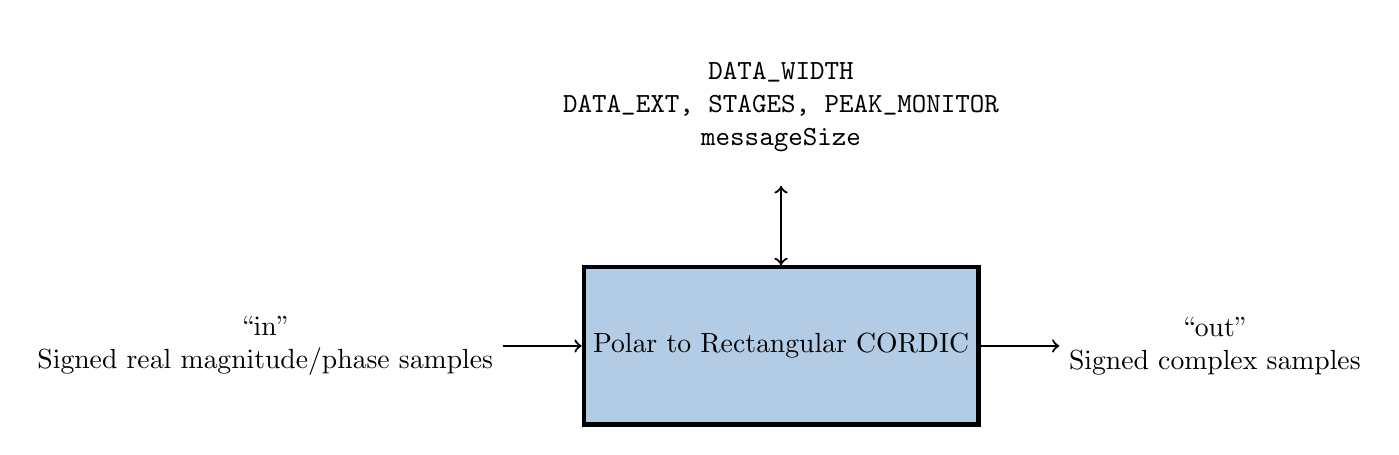
\begin{tikzpicture}[% List of styles applied to all, to override specify on a case-by-case
			every node/.style={
				align=center,  		% use this so that the "\\" for line break works
				minimum size=2cm	% creates space above and below text in rectangle
			},
			every edge/.style={draw,thick}
		]
		\node[rectangle,ultra thick,draw=black,fill=blue](R2){\Comp};
		\node[rectangle,draw=white,fill=white](R3)[left= of R2]{``in'' \\ Signed real magnitude/phase samples};
		\node[rectangle,draw=white,fill=white](R4)[right= of R2]{``out'' \\ Signed complex samples};
		\node[rectangle,draw=white,fill=white](R5)[above= of R2]{\verb+DATA_WIDTH+ \\ \verb+DATA_EXT, STAGES, PEAK_MONITOR+ \\ \verb+messageSize+};
		\path[->]
		(R3)edge []	node [] {} (R2)
		(R2)edge []	node [] {} (R4)
		(R2)edge []	node [] {} (R5)
		(R5)edge []	node [] {} (R2)
		;
	\end{tikzpicture}
\end{center}

\subsection*{State Machine}
None

\newpage

\section*{Source Dependencies}
\subsection*{\comp.hdl}
\begin{itemize}
	\item projects/assets/components/dsp\_comps/pr\_cordic.hdl/pr\_cordic.vhd
	\item projects/assets/hdl/primitives/dsp\_prims/dsp\_prims\_pkg.vhd
	      \subitem projects/assets/hdl/primitives/dsp\_prims/cordic/src/cordic\_pr.vhd
	      \subitem projects/assets/hdl/primitives/dsp\_prims/cordic/src/cordic.vhd
	      \subitem projects/assets/hdl/primitives/dsp\_prims/cordic/src/cordic\_stage.vhd
	\item projects/assets/hdl/primitives/misc\_prims/misc\_prims\_pkg.vhd
	      \subitem projects/assets/hdl/primitives/misc\_prims/round\_conv/src/round\_conv.vhd
	\item projects/assets/hdl/primitives/util\_prims/util\_prims\_pkg.vhd
	      \subitem projects/assets/hdl/primitives/util\_prims/pd/src/peakDetect.vhd
\end{itemize}

\begin{landscape}
	\section*{Component Spec Properties}
	\begin{scriptsize}
		\begin{tabular}{|p{3cm}|p{1.5cm}|c|c|c|c|c|p{7cm}|}
			\hline
			\rowcolor{blue}
			Name                & Type   & SequenceLength & ArrayDimensions & Accessibility      & Valid Range & Default & Usage                                    \\
			\hline
			\verb+DATA_WIDTH+   & UChar  & -              & -               & -          & -           & -       & Real input and complex output data width \\
			\hline
			\verb+DATA_EXT+     & UChar  & -              & -               & -          & -           & -       & CORDIC requirement: Number of growth bits implemented by CORDIC \\
			\hline
			\verb+STAGES+       & UChar  & -              & -               & -          & -           & -       & Number of CORDIC stages implemented \\
			\hline
			\verb+messageSize+ & UShort & -              & -               & Writable & 8192        & 8192    & Number of bytes in output message (Not implemented by Version 2)\\
			\hline
		\end{tabular}
	\end{scriptsize}

	\section*{Worker Properties}
	\subsection*{\comp.hdl}
	\begin{scriptsize}
		\begin{tabular}{|p{2cm}|p{1.5cm}|c|c|c|c|c|c|p{7cm}|}
			\hline
			\rowcolor{blue}
			Type         & Name              & Type & SequenceLength & ArrayDimensions & Accessibility & Valid Range & Default & Usage                                    \\
			\hline
			SpecProperty & \verb+DATA_WIDTH+ & -    & -              & -               & Parameter     & 1-16        & 16      & Real input and complex output data width \\
			\hline
			SpecProperty & \verb+DATA_EXT+   & -    & -              & -               & Parameter     & 1-16        & 6      & CORDIC requirement: \# of extension bits \\
			\hline
			SpecProperty & \verb+STAGES+     & -    & -              & -               & Parameter     & 16-32       & 18      & Number of CORDIC stages implemented      \\
			\hline
			Property & \verb+PEAK_MONITOR+     & Bool     & -              & -               & Parameter     & Standard        & true      & Enable/Disable build-time inclusion of peak monitoring \\
			\hline
			Property     & \verb+peak+  & Short & -              & -               & Volatile      & Standard    & -       & Peak value of FM Discriminator output \\
			\hline
		\end{tabular}
	\end{scriptsize}

	\section*{Component Ports}
	\begin{scriptsize}
		\begin{tabular}{|M{2cm}|M{1.5cm}|M{4cm}|c|c|M{9cm}|}
			\hline
			\rowcolor{blue}
			Name & Producer & Protocol           & Optional & Advanced & Usage                  \\
			\hline
			in   & false    & iqstream\_protocol & false    & -        & Signed complex (Magnitude/Phase) samples \\
			\hline
			out  & true     & iqstream\_protocol & false    & -        & Signed complex (I/Q) samples \\
			\hline
		\end{tabular}
	\end{scriptsize}

	\section*{Worker Interfaces}
	\subsection*{\comp.hdl}
	\begin{scriptsize}
		\begin{tabular}{|M{2cm}|M{1.5cm}|c|c|M{12cm}|}
			\hline
			\rowcolor{blue}
			Type            & Name & DataWidth & Advanced 					 & Usage                  \\
			\hline
			StreamInterface & in   & 32        & - & Signed magnitude samples (31:16), Signed phase samples (15:0) \\
			\hline
			StreamInterface & out  & 32        & InsertEOM=1 & Signed complex samples \\
			\hline
		\end{tabular}
	\end{scriptsize}
\end{landscape}

\section*{Control Timing and Signals}
The CORDIC Polar-to-Rectangular HDL worker uses the clock from the Control Plane and standard Control Plane signals. This worker has a start-up transient delay of \verb+STAGES++2 valid samples. This means that once the input is ready and valid and the output is ready, it takes that many valid input samples before the first output sample is made available. The delays for this worker are itemized be as follows:
\begin{itemize}
	\item 0 : pr\_cordic.vhd
	\item 1 : pr\_cordic.vhd/cordic\_pr.vhd
	\item STAGES : pr\_cordic.vhd/cordic\_pr.vhd/cordic.vhd/cordic\_stage.vhd
	\item 1 : cordic\_pr.vhd/round\_conv.vhd
\end{itemize}

\begin{tabular}{|M{4.5cm}|M{1cm}|M{1cm}|M{1.5cm}|M{2cm}|M{1cm}|M{1cm}|M{2.5cm}|}
	\hline
	\rowcolor{blue}
	Latency                      \\
	\hline
	\verb+STAGES++2 clock cycles \\
	\hline
\end{tabular}


\begin{landscape}
\section*{Worker Configuration Parameters}
\subsubsection*{\comp.hdl}
%\input{../../\ecomp.hdl/configurations.inc}
\section*{Performance and Resource Utilization}
\subsubsection*{\comp.hdl}
%\input{../../\ecomp.hdl/utilization.inc}
\end{landscape}
\section*{Test and Verification}
\begin{flushleft}
	A single test case is implemented to validate the CORDIC Polar-to-Rectangular component. An input file is generated with a constant magnitude of 29760 in bits (31:16) (driven into CORDIC input $x_0$) and multiple cycles of ramp data centered about zero representing a constant phase in bits (15:0) (driven into CORDIC input $z_0$). The amount of input data was chosen such that, at least two messages were output. The expected outputs are a cosine from $I$ (the CORDIC $x_N$ output) with a magnitude equal to that of $x_0$ and a sine from $Q$ (the CORDIC $y_N$ output) also with a magnitude equal to that of $x_0$. Input magnitude and phase plots may be viewed in Figures \ref{fig:input_magnitude} and \ref{fig:input_phase} below.
\end{flushleft}

	\begin{figure}[ht]
		\centering
		\begin{minipage}{.5\textwidth}
			\centering\includegraphics[width=1.0\linewidth]{input_magnitude}
			\captionof{figure}{Time Domain Magnitude Input}
			\label{fig:input_magnitude}
		\end{minipage}%
		\begin{minipage}{.5\textwidth}
			\centering\includegraphics[width=1.0\linewidth]{input_phase}
			\captionof{figure}{Time Domain Phase Input}
			\label{fig:input_phase}
		\end{minipage}
	\end{figure}

\begin{flushleft}
	Verification of output data is performed by creating cycles of a complex sinusoid in python to match the expected number of output data, and then comparing the worker output sample-by-sample with these expected results. A difference of $\pm1.0$ is tolerated to allow for differences in fixed-point implementation and hardware rounding. Figures \ref{fig:output_time} and \ref{fig:output_freq} depict the output of the Polar to Rectangular CORDIC.
\end{flushleft}

	\begin{figure}[ht]
		\centering
		\begin{minipage}{.5\textwidth}
			\centering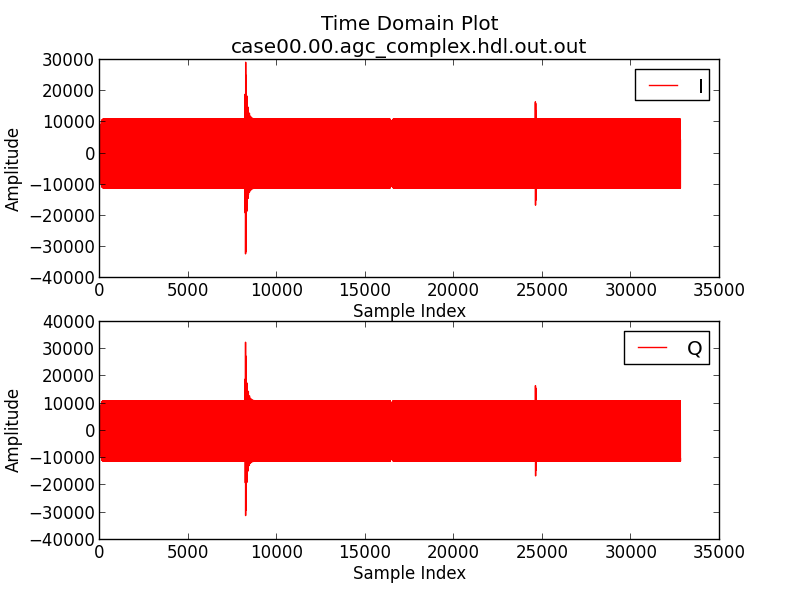
\includegraphics[width=1.0\linewidth]{output_time}
			\captionof{figure}{Time Domain Rectangular Output}
			\label{fig:output_time}
		\end{minipage}%
		\begin{minipage}{.5\textwidth}
			\centering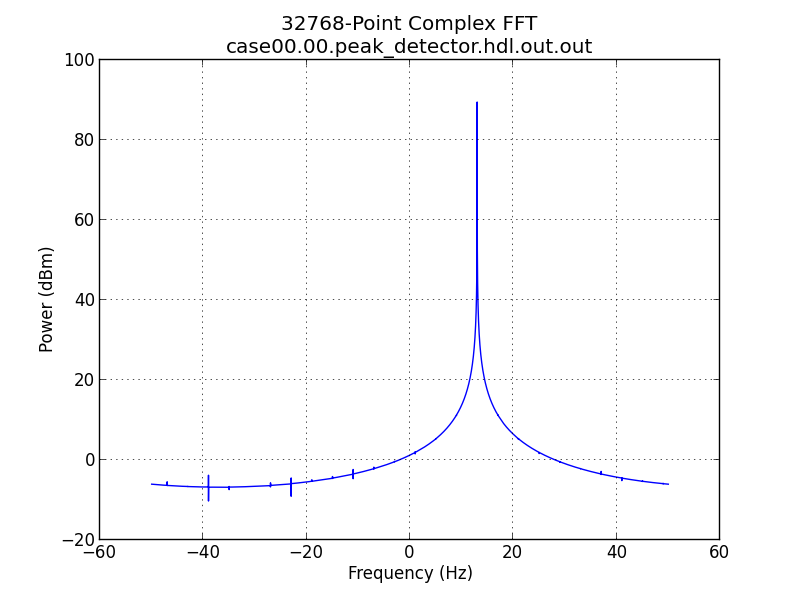
\includegraphics[width=1.0\linewidth]{output_freq}
			\captionof{figure}{Frequency Domain Rectangular Output}
			\label{fig:output_freq}
		\end{minipage}
	\end{figure}

\end{document}
